% Architecture diagram (compiled separately to fig_architecture.pdf)
\documentclass[tikz,border=4pt]{standalone}
\usepackage[T1]{fontenc}
\usepackage{lmodern}
\usetikzlibrary{arrows.meta,positioning,fit,backgrounds,calc}
\begin{document}
\sffamily\footnotesize
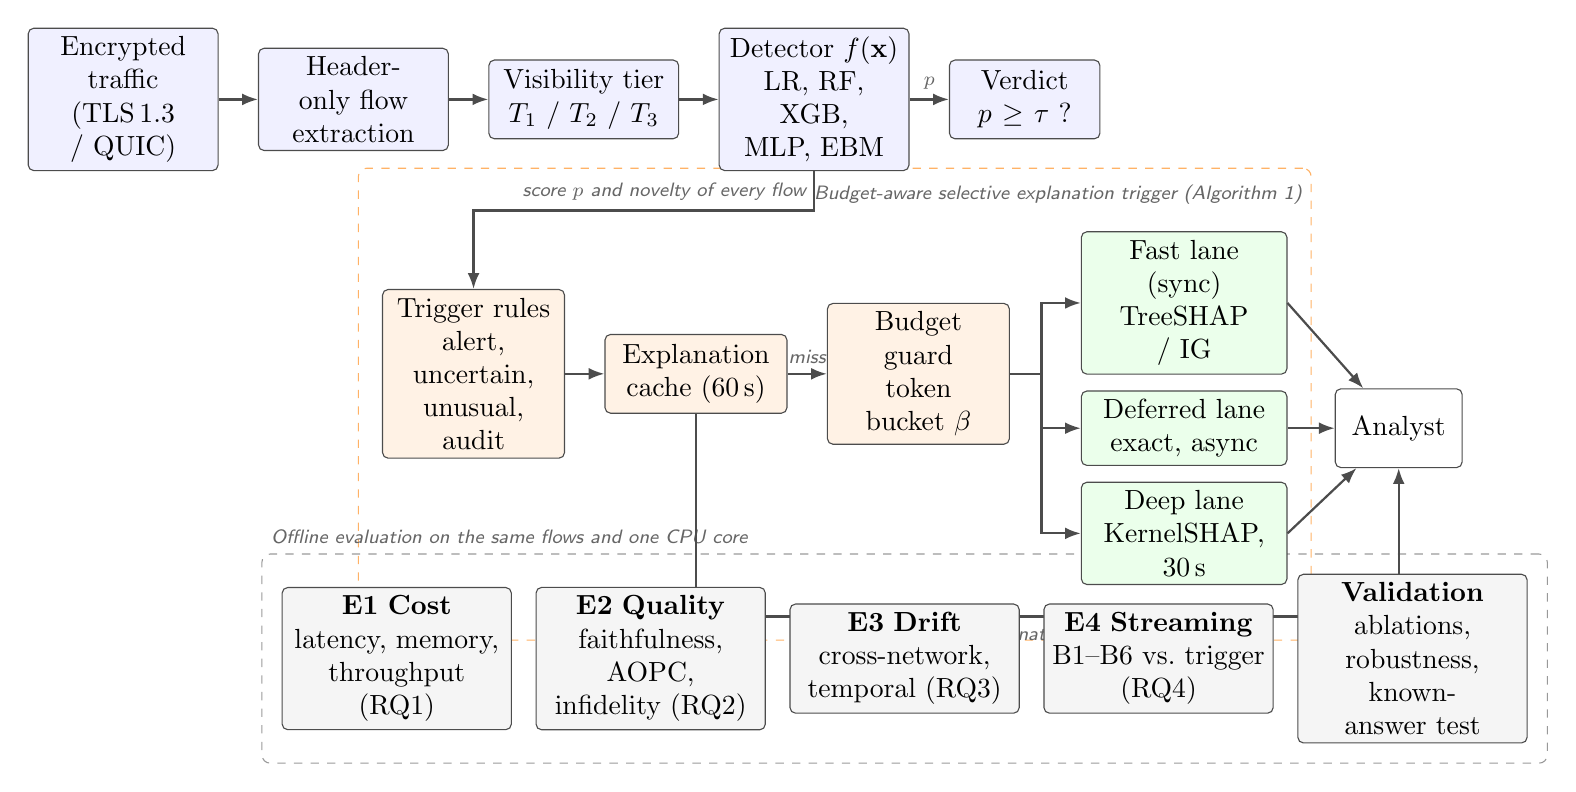
\begin{tikzpicture}[
  box/.style={draw=black!70, rounded corners=2pt, align=center, minimum height=10mm, inner sep=3pt, fill=white},
  pipe/.style={box, fill=blue!6, text width=22mm},
  trig/.style={box, fill=orange!10, text width=21mm},
  lane/.style={box, fill=green!8, text width=24mm, minimum height=8mm},
  eval/.style={box, fill=black!4, text width=27mm, minimum height=12mm},
  arr/.style={-{Latex[length=2mm]}, thick, black!70},
  lbl/.style={font=\sffamily\scriptsize\itshape, black!60}
]
% ---------------- online pipeline ----------------
\node[pipe] (traffic) {Encrypted traffic\\(TLS\,1.3 / QUIC)};
\node[pipe, right=5mm of traffic] (extract) {Header-only flow\\extraction};
\node[pipe, right=5mm of extract] (tier) {Visibility tier\\$T_1$ / $T_2$ / $T_3$};
\node[pipe, right=5mm of tier] (det) {Detector $f(\mathbf{x})$\\LR, RF, XGB, MLP, EBM};
\node[pipe, right=5mm of det, text width=17mm] (verdict) {Verdict\\$p \ge \tau$ ?};
\draw[arr] (traffic) -- (extract);
\draw[arr] (extract) -- (tier);
\draw[arr] (tier) -- (det);
\draw[arr] (det) -- node[above, lbl] {$p$} (verdict);

% ---------------- trigger ----------------
\node[trig, below=19mm of tier, xshift=-14mm] (rules) {Trigger rules\\alert, uncertain,\\unusual, audit};
\node[trig, right=5mm of rules] (cache) {Explanation\\cache (60\,s)};
\node[trig, right=5mm of cache] (budget) {Budget guard\\token bucket $\beta$};
\node[lane, right=9mm of budget, yshift=9mm] (fast) {Fast lane (sync)\\TreeSHAP / IG};
\node[lane, below=2mm of fast] (deferred) {Deferred lane\\exact, async};
\node[lane, below=2mm of deferred] (deep) {Deep lane\\KernelSHAP, 30\,s};
\node[box, right=6mm of deferred, text width=14mm, fill=white] (analyst) {Analyst};
\draw[arr] (det.south) -- ++(0,-5mm) -| node[pos=0.22, above, lbl] {score $p$ and novelty of every flow} (rules.north);
\draw[arr] (rules) -- (cache);
\draw[arr] (cache) -- node[above, lbl] {miss} (budget);
\draw[arr] (budget.east) -- ++(4mm,0) |- (fast.west);
\draw[arr] (budget.east) -- ++(4mm,0) |- (deferred.west);
\draw[arr] (budget.east) -- ++(4mm,0) |- (deep.west);
\draw[arr] (fast.east) -- (analyst);
\draw[arr] (deferred.east) -- (analyst);
\draw[arr] (deep.east) -- (analyst);
\coordinate (hitlow) at ($(deep.south)+(0,-4mm)$);
\coordinate (fasttop) at ($(fast.north)+(0,5mm)$);
\draw[arr] (cache.south) |- node[pos=0.75, below, lbl] {hit: reuse a recent explanation} (hitlow) -| (analyst.south);
\begin{scope}[on background layer]
  \node[draw=orange!60, dashed, rounded corners=3pt, fit=(rules)(cache)(budget)(fast)(deep)(hitlow)(fasttop), inner sep=3mm,
        label={[lbl, anchor=north east, yshift=-1mm]north east:Budget-aware selective explanation trigger (Algorithm~1)}] (trigbox) {};
\end{scope}

% ---------------- offline evaluation ----------------
\node[eval, below=22mm of cache, xshift=-38mm] (e1) {\textbf{E1 Cost}\\latency, memory,\\throughput (RQ1)};
\node[eval, right=3mm of e1] (e2) {\textbf{E2 Quality}\\faithfulness, AOPC,\\infidelity (RQ2)};
\node[eval, right=3mm of e2] (e3) {\textbf{E3 Drift}\\cross-network,\\temporal (RQ3)};
\node[eval, right=3mm of e3] (e4) {\textbf{E4 Streaming}\\B1--B6 vs.\ trigger\\(RQ4)};
\node[eval, right=3mm of e4] (e5) {\textbf{Validation}\\ablations, robustness,\\known-answer test};
\begin{scope}[on background layer]
  \node[draw=black!40, dashed, rounded corners=3pt, fit=(e1)(e5), inner sep=2.5mm,
        label={[lbl, anchor=south west]north west:Offline evaluation on the same flows and one CPU core}] (evalbox) {};
\end{scope}
\end{tikzpicture}
\end{document}
